

Mithilfe von Scopes oder Plots werden nun die gesuchten Signale abgegriffen und als Funktionen der Zeit dargestellt. \\
Die Abbildungen \ref{fig:Moment}, \ref{fig:Omega} und \ref{fig:StreckeundUnwuchtkraft} sind Plots aus Matlab, die wie folgt definiert wurden:

\begin{figure}[hbt]
	\centering
	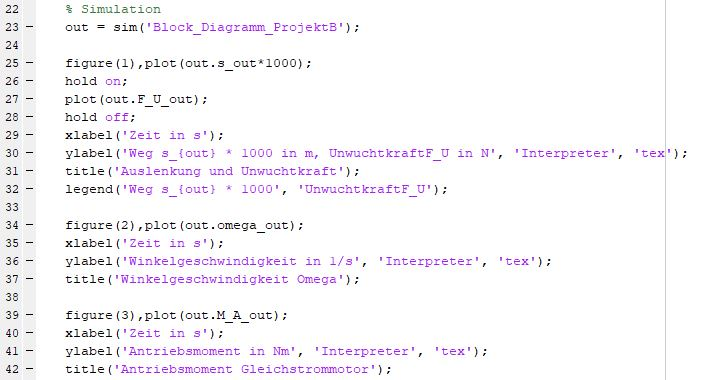
\includegraphics[width=1\linewidth]{Images/Simulationscode}
	\caption{Codeausschnitt aus dem Workspace zur Definition der Plots}
	\label{fig:Simcode}
\end{figure}

In den folgenden Abbildungen \ref{fig:Moment}, \ref{fig:Omega} und \ref{fig:StreckeundUnwuchtkraft} sind das Motormoment $M$, die Winkelgeschwindigkeit $\Omega$, die Strecke $s$ und die Unwuchtkraft $F_U$ über die Zeit von $100 \milli\second$ dargestellt. Für kleine Änderungen der Dämpfungskonstanten können die translatorischen und rotatorischen Bewegungsgleichungen getrennt betrachtet werden.

\begin{figure}[hbt]
	\centering
	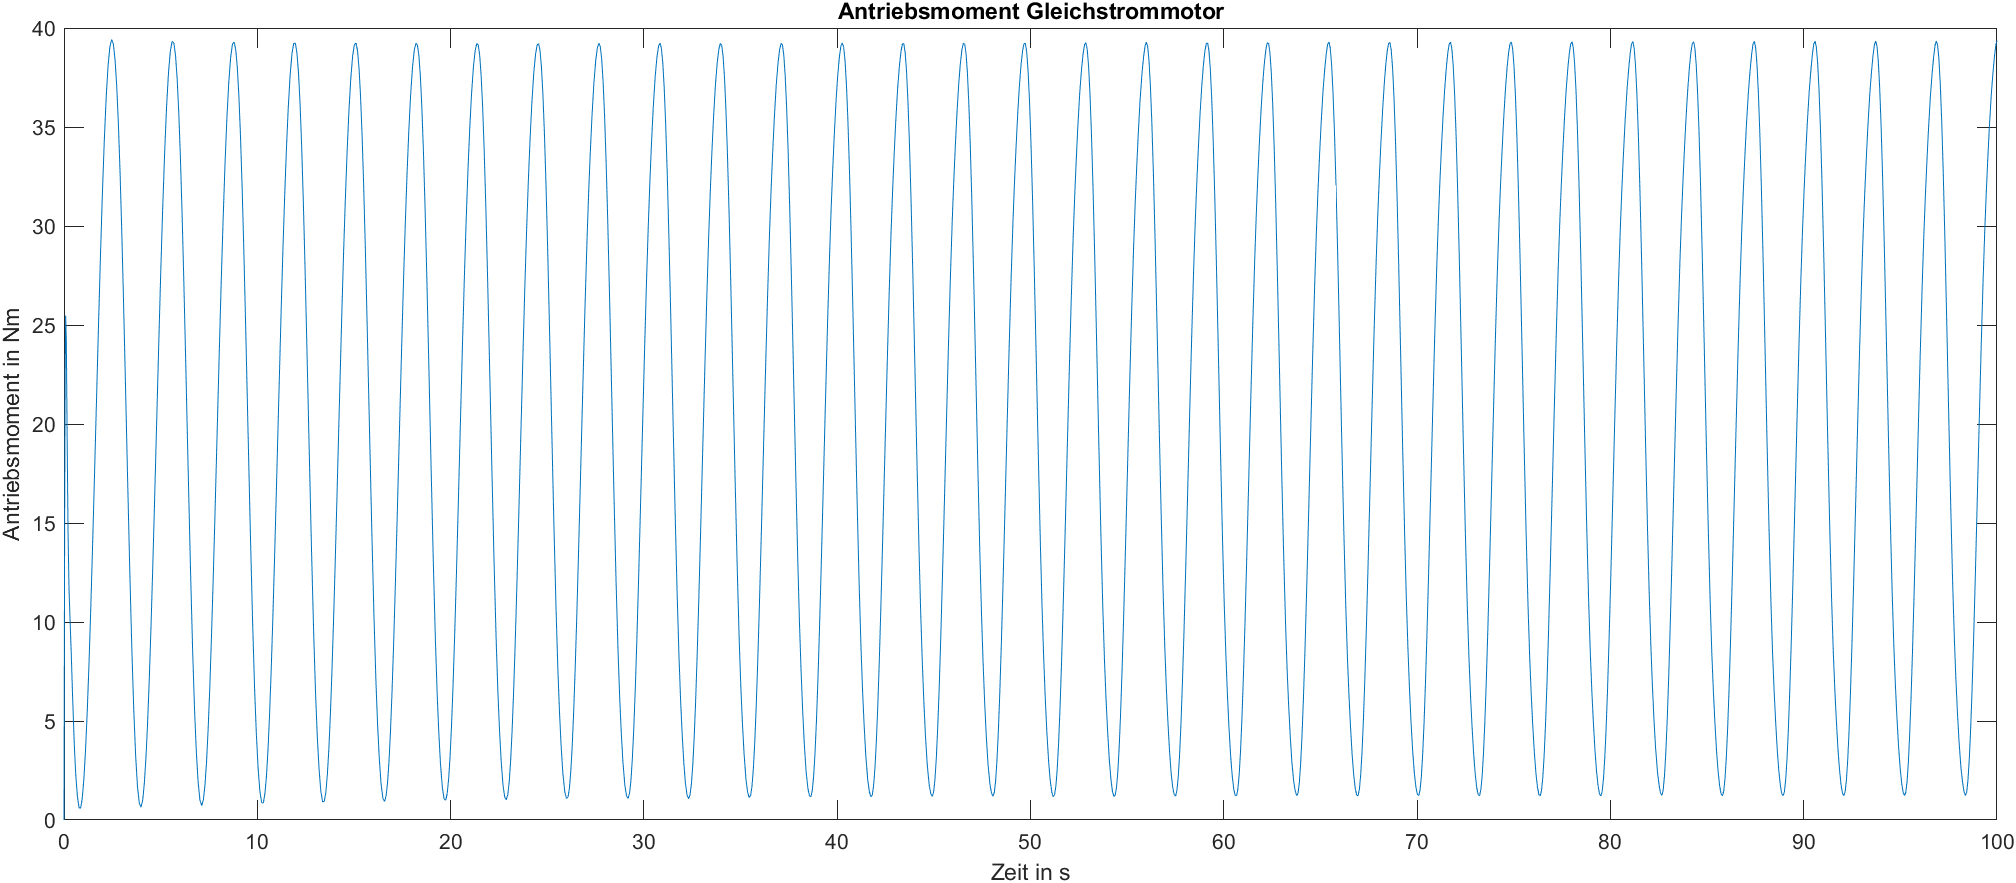
\includegraphics[width=1\linewidth]{Images/Moment}
	\caption{Simulationsergebnis: Antriebsmoment des Gleichstrommotors}
	\label{fig:Moment}
\end{figure}

Das in Abbildung \ref{fig:Moment} dargestellte Antriebsmoment ist hauptsächlich abhängig von der rotatorischen Bewegungsgleichung des Schwingsystems, ebenso wie die Winkelgeschwindigkeit $\Omega$. Im Verlauf dieser beiden Größen und aus dem gegebenen Parametersatz kann dieses Teilsystem dem Schwingfall zugewiesen werden, dessen zeitlicher Verlauf auf eine ungedämpfte Schwingung deuten lässt und damit auch auf die Grenzstabilität des Systems. Zur genaueren Analyse, wird der Wert der rotatorischen Dämpfungskonstante $d_r$ verändert, um die Abhängigkeit von dieser zu überprüfen. 
Verdoppelt man den Wert von $d_r$ verschiebt sich die Amplitude des Antriebsmoments um $20 \newton\meter$ nach oben. Bei einer weiteren Erhöhung wird die Kurve ebenfalls immer weiter nach oben gerückt, wobei sich jedoch die Amplitude von $40 \newton\meter$ kaum verändert. \\
Unter den Standardbedingungen befindet sich die Winkelgeschwindigkeit zwischen $1,85 \frac{1}{\second}$ und $2,18 \frac{1}{\second}$. Die Veränderungen an der Dämpfungskonstante $d_r$ hatten keinen nennenswerten Einfluss auf die Winkelgeschwindigkeit. Um diese marginal zu Beeinflussen müsste entweder die Motorkonstante $K_A$ angepasst werden, was sich wiederum auf das Antriebsmoment und die Unwuchtkraft auswirkt, oder $d_t$ wird größer gewählt wodurch der Maximalwert von $\Omega$ verkleinert wird. \\

\newpage

\begin{figure}[hbt]
	\centering
	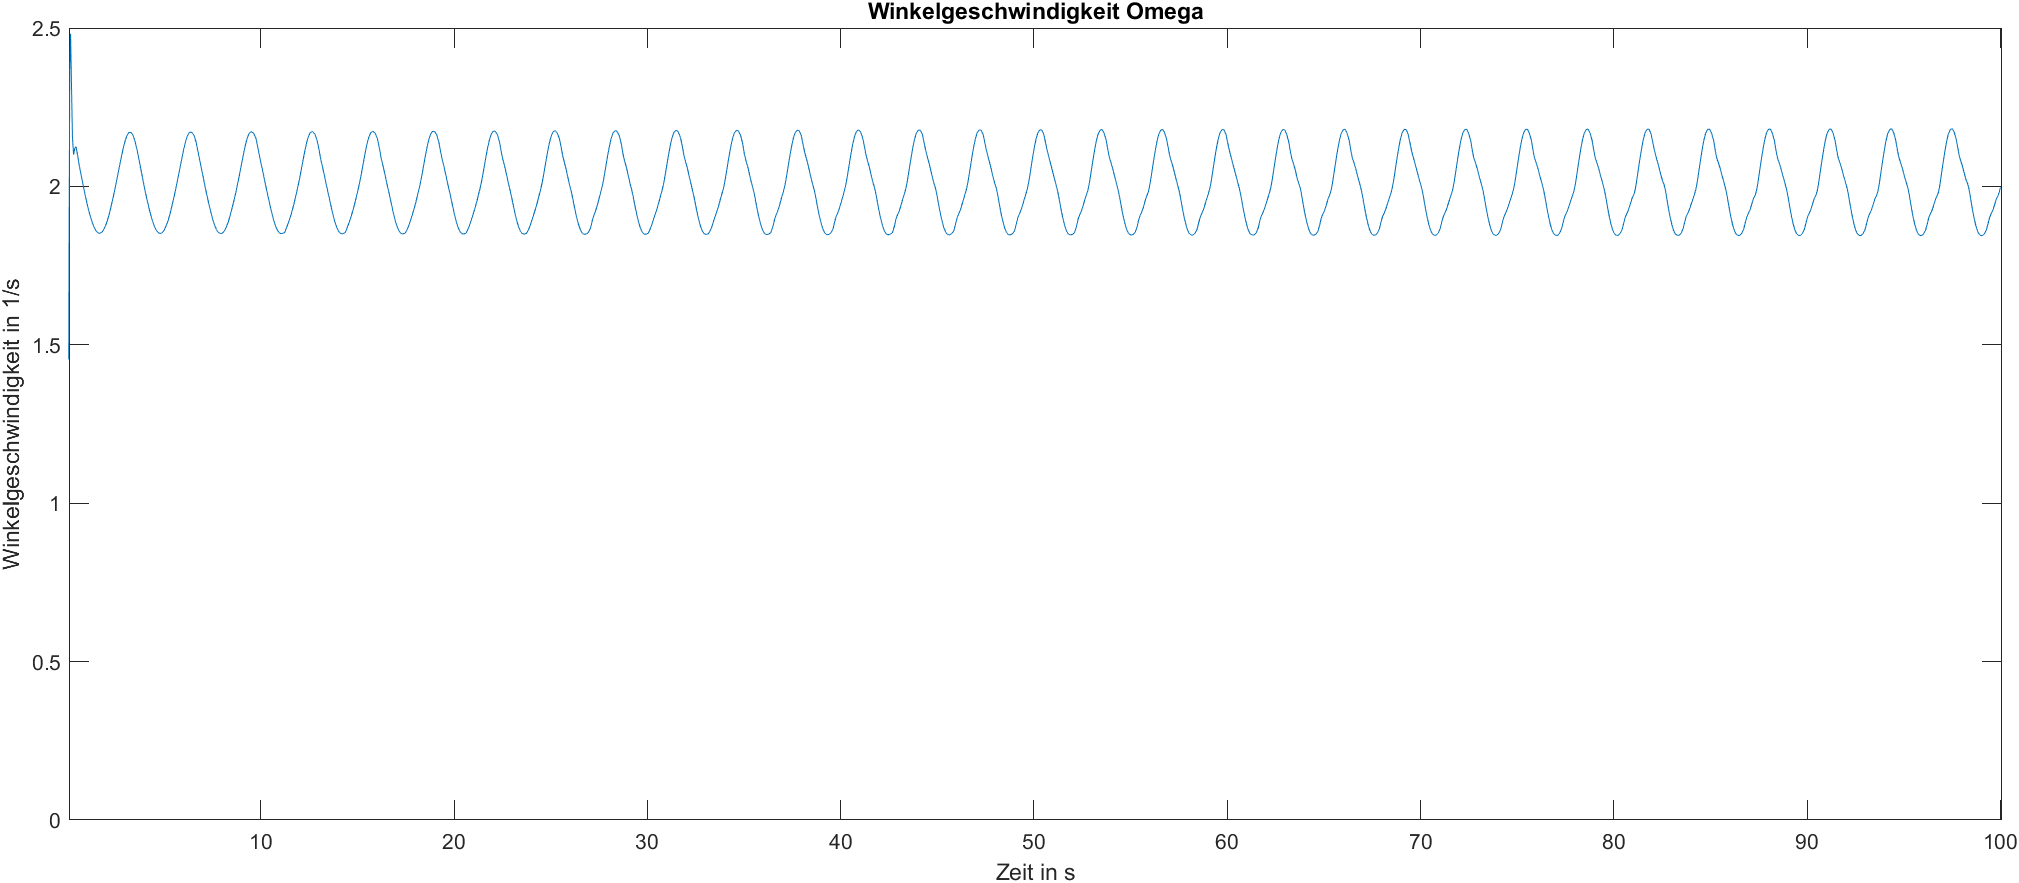
\includegraphics[width=1\linewidth]{Images/Omega}
	\caption{Simulationsergebnis: Winkelgeschwindigkeit des mechatronischen Systems}
	\label{fig:Omega}
\end{figure}

Auffällig ist in Abbildung \ref{fig:StreckeundUnwuchtkraft}, dass die Auslenkung die doppelte Frequenz der Unwuchtkraft hat. Für die Auslenkung und Unwuchtkraft des Systems ist vor allem die translatorische Bewegungsgleichung verantwortlich. Aus Abbildung \ref{fig:StreckeundUnwuchtkraft} ist ersichtlich, dass es sich bei diesem Teilsystem um einen Schwingfall handelt. Im weiteren lässt der zeitliche Verlauf beider Kurven auf zwei unterschiedliche Schwingungsverhalten schließen. Die Amplitude der Auslenkung zeigt ein ungedämpftes Verhalten, wodurch diese Teilgleichung als instabil klassifiziert werden kann. Dahingegen zeigt der Graph von $F_U$ eine ungedämpfte Schwingung, bei gleichbleibender Amplitude und damit Eigenschaften eines grenzstabilen Systems. Um eine detailliertere Aussage über das translatorische System zu treffen wird dessen Dämpfungskonstante $d_t$ variiert. \\
Bei einer Erhöhung wird die Amplitude im gleichen Zeitbereich verkleinert. Je höher $d_t$ gewählt wird, desto kleiner wird die Amplitude der Auslenkung. Der resultierende Graph lässt darauf deuten, dass sich die Schwingung einem stabilen, ungedämpftem System annähert. Die Unwuchtkraft zeigt keine Reaktion auf die veränderten Werte der Dämpfungskonstante, ebenso wie $M_A$ und $\Omega$. \\

\newpage

\begin{figure}[hbt]
	\centering
	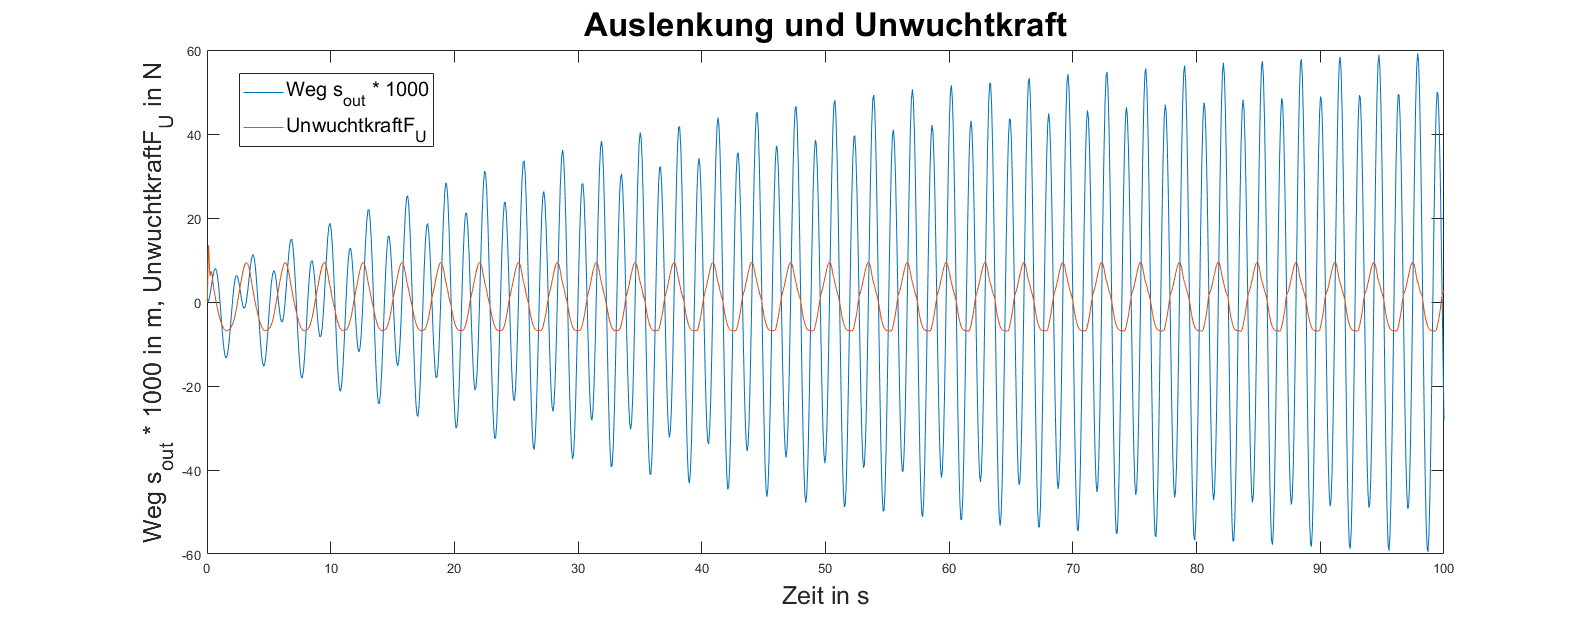
\includegraphics[width=1\linewidth]{Images/StreckeundUnwuchtkraft}
	\caption{Simulationsergebnis: Auslenkung$\cdot$1000 und Unwuchtkraft des mechatronischen Systems}
	\label{fig:StreckeundUnwuchtkraft}
\end{figure}

Für beide Teilsysteme gilt, dass sie in erster Linie von ihren Dämpfungskonstanten abhängig sind und sich dadurch nicht marginal gegenseitig beeinflussen, solange diese nicht extrem groß werden. Lässt man $d_r$ gegen einen großen Wert laufen verkleinert sich die Amplitude von $F_U$, zugleich nähert sich der Auslenkungsgraph, dem von $F_U$ in Frequenz und Schwingungsverlauf an. Im anderen Teilsystem lässt sich beim Antriebsmoment keine Schwingung mehr erkennen, dieses läuft gegen einen Grenzwert. Vergleichbar vom Signalverlauf verhält sich auch die Winkelgeschwindigkeit, welche anfangs linear ansteigt und letztlich mit kleiner Amplitude um einen Wert schwingt. Wird $d_t$ sehr groß, hat das keine Auswirkungen auf $M_A$, $\Omega$ und $F_U$, nur die Auslenkung wird dadurch beeinflusst. Diese verhält sich ähnlich zur vorherigen Grenzbetrachtung und schmiegt sich zunächst $F_U$ an. Im weiteren Verlauf verringert sich die Amplitude der Auslenkung jedoch weiter und die der Unwuchtkraft bleibt gleich.